\chapter{Setting the Stage: Core Mathematics of Deep Learning}
\begin{mdframed}[linewidth=1pt, linecolor=gray, backgroundcolor=gray!5] \vspace{0.2cm} \textbf{\Large After finishing this chapter, you will know:} \vspace{0.1cm}

\begin{itemize}[label=\textbf{\textendash}, leftmargin=1.5em, itemsep=0.5em, labelsep=0.5em] \item \textit{How neural networks work}: Get introduced to the structure and function of neural networks through a practical example. \item \textit{The role of tensors}: Understand tensors as the core data structures for deep learning and their representations. \item \textit{Tensor operations}: Explore foundational operations like element-wise computations, broadcasting, and reshaping, which drive neural network computations. \item \textit{How neural networks learn}: Grasp the concept of backpropagation and how optimization techniques like gradient descent enable learning. \item \textit{Connecting the dots}: See how these mathematical principles come together in a real-world example. \end{itemize} \vspace{0.2cm} \end{mdframed}


Deep learning, at its core, is about building powerful models that learn to represent and predict patterns from data. However, to truly harness its potential, you need to understand the mathematical concepts that underlie it. In this chapter, we’ll gently introduce you to these foundational ideas—without overwhelming you with unnecessary mathematical jargon.

By the end of this chapter, you’ll have a strong intuition about key mathematical building blocks like tensors, operations on tensors, and gradient-based optimization techniques. We’ll walk you through practical examples, starting with a simple neural network for a drought classification task. This example will anchor our exploration of mathematical concepts such as tensors, tensor operations, gradients, and optimization.

% \begin{enumerate}
%     \item \textbf{Introducing Neural Networks Through an Example:}We begin with a hands-on example: predicting whether a region is experiencing a drought. This practical task will introduce the fundamental ideas behind neural networks and set the stage for the deeper concepts to come.


%     \item \textbf{How Neural Networks Learn: Optimization Basics:}Dive into the mechanisms that drive learning in neural networks. We’ll explore how gradients and derivatives play a critical role in adjusting the model's parameters and introduce gradient-based optimization, including the concept of backpropagation, which powers the training process.

% \item \textbf{Putting It All Together:} After building your understanding of the core principles, we’ll revisit the drought classification example to see how these concepts work in practice. This section will reinforce your learning and prepare you for applying these ideas to real-world problems in upcoming chapters.
% \end{enumerate}
\section{Introducing Neural Networks Through a Simple Example: Drought Classification}
\section{Understanding Tensors: The Data Structures of Deep Learning}

At the heart of deep learning lies the concept of \textbf{tensors}—fundamental data structures that store and process information in neural networks. If you’ve worked with arrays or matrices before, tensors will feel familiar, as they generalize these structures to higher dimensions. Tensors are especially useful in hydrology because they can represent diverse data types across spatial, temporal, and physical dimensions.

Tensors are versatile and can handle data in various shapes and sizes, from single numbers to multidimensional arrays like images or time-series datasets. Their ability to handle multidimensional data makes them the backbone of modern deep learning frameworks like TensorFlow and PyTorch.

\subsection{What is a Tensor?}

A tensor is essentially a container for numerical data. While matrices (two-dimensional arrays) are a familiar example, tensors extend this concept to an arbitrary number of dimensions. Each tensor has three key attributes:

\begin{itemize}
    \item \textbf{Number of axes (rank):} The rank indicates how many dimensions the tensor has. For example, a scalar (single value) has no axes, a vector has one axis, and a matrix has two axes (rows and columns).
    \item \textbf{Shape:} The shape describes the number of elements along each axis. For instance, a matrix with three rows and four columns has a shape of \textit{(3, 4)}.
    \item \textbf{Data type (dtype):} This specifies the type of data stored in the tensor, such as integers (\texttt{int32}) or floating-point numbers (\texttt{float64}).
\end{itemize}

\subsection{Different Types of Tensors}
\begin{enumerate}
    \item \textbf{Scalars (0D Tensors):} Scalars are the simplest type of tensor, containing a single value with no axes.
    \begin{lstlisting}[language=Python]
    import numpy as np
    scalar = np.array(5)
    print(scalar.ndim)  # Output: 0
    \end{lstlisting}
    \textit{In hydrology, scalars might represent constants, such as the threshold for drought classification.}

    \item \textbf{Vectors (1D Tensors):} A vector is a one-dimensional array of numbers, often used to represent features of a single sample.
    \begin{lstlisting}[language=Python]
vector = np.array([45.2, 18.3, 0.35, 6.4])  # Precipitation, temp, soil moisture, evaporation
print(vector.ndim)  # Output: 1
    \end{lstlisting}
    \textit{Example: Each vector could represent features of a specific location for streamflow prediction, such as precipitation (mm), temperature (°C), soil moisture (\%), and evaporation (mm/day). A dataset with 1,000 such samples would form a 2D tensor of shape \texttt{(1000, 4)}.}

    \item \textbf{Matrices (2D Tensors):} A matrix is a two-dimensional tensor, often representing tabular datasets.
    \begin{lstlisting}[language=Python]
matrix = np.array([[1, 2, 3], [4, 5, 6], [7, 8, 9]])
print(matrix.ndim)  # Output: 2
    \end{lstlisting}
    \textit{Example: A table of daily river discharge values across multiple monitoring stations could be stored as a matrix, where rows represent days and columns represent stations.}

    \item \textbf{3D Tensors and Beyond:} Higher-dimensional tensors are created by stacking lower-dimensional tensors along new axes.
    \begin{lstlisting}[language=Python]
tensor_3d = np.array([
    [[1, 2], [3, 4]],
    [[5, 6], [7, 8]]
])
print(tensor_3d.ndim)  # Output: 3
    \end{lstlisting}
    \textit{Example: A 3D tensor might store rainfall data as grids over a region, with axes for latitude, longitude, and time. For satellite images, a 4D tensor might represent a batch of images with dimensions \texttt{(number of images, height, width, channels)}.}
\end{enumerate}

\begin{tcolorbox}[enhanced,
  watermark opacity=0.3,watermark zoom=0.9,
  colback=blue!5!white, colframe=blue!70!black,
  fonttitle=\bfseries, title=Do you know? ]
Images are often used in hydrology to represent spatial data, such as land cover, satellite images, or digital elevation models (DEMs). These are stored as 3D tensors with dimensions for height, width, and color channels.

\textbf{Flood Mapping with Satellite Images}  
\begin{itemize}
    \item  A grayscale satellite image of a flood-affected area is stored as a 3D tensor of shape \texttt{(256, 256, 1)}.
    \item  For RGB images (e.g., land cover classification), the shape becomes \texttt{(256, 256, 3)}, with three color channels (red, green, blue).
\end{itemize}

To process a batch of 100 such images, we use a 4D tensor with shape \texttt{(100, 256, 256, 3)}, where the first dimension represents the number of images.
\end{tcolorbox}



\subsection{Why Tensors Are Crucial for Hydrological Models}

Hydrological data is inherently multi-dimensional, making tensors a natural choice for data representation. Here’s why tensors are indispensable in hydrology:
\begin{itemize}
    \item \textbf{Handling Diverse Data:} Tensors allow seamless processing of both numerical vectors (e.g., precipitation and temperature) and spatial data (e.g., satellite imagery).
    \item \textbf{Capturing Spatiotemporal Relationships:} Tensors represent time-series data, spatial grids, and their interactions, enabling models to learn dependencies across time and space.
\end{itemize}


\subsection{Tensor Slicing and Indexing}

Tensors, as flexible data structures, allow for efficient manipulation through operations like slicing and indexing. These operations enable us to extract, reshape, and process relevant subsets of data. For water scientists, such operations are crucial for tasks like analyzing subsets of spatial grids, extracting temporal patterns, or managing large datasets like satellite imagery or time-series records.
Tensor slicing is a way to extract specific portions of a tensor by specifying start and end indices along each axis. This is particularly useful when working with large datasets, such as remote sensing imagery or time-series data.

\begin{itemize}
    \item \textbf{Example 1: Extracting a Subset of Remote Sensing Data}
    Consider a tensor representing a 3D satellite image of shape \texttt{(256, 256, 3)} (height, width, and RGB channels).
\begin{lstlisting}[language=Python]
import numpy as np
image = np.random.random((256, 256, 3))  # A random image
# Extract a 100x100 patch from the top-left corner
patch = image[:100, :100, :]
print(patch.shape)  # Output: (100, 100, 3)
\end{lstlisting}
You can also extract specific regions using negative indices, which count backward from the end of an axis:
\begin{lstlisting}[language=Python]
# Extract a 50x50 patch from the bottom-right corner
bottom_patch = image[-50:, -50:, :]
print(bottom_patch.shape)  # Output: (50, 50, 3)
\end{lstlisting}
\end{itemize}
\subsection{Batching Data for Training}

Deep learning models process data in batches rather than all at once. The first axis of a tensor typically represents the batch axis, where each element corresponds to one sample.
\begin{itemize}
    \item \textbf{Example 2: Preparing Batches of Rainfall Data}
    Consider a dataset of daily rainfall records for 1,000 locations over 365 days. This data can be represented as a 3D tensor of shape \texttt{(1000, 365, 1)} (locations, days, and rainfall amount):


\begin{lstlisting}[language=Python]
# Dataset with random rainfall data
rainfall_data = np.random.random((1000, 365, 1))
# Extract the first batch of 128 locations
batch = rainfall_data[:128]
print(batch.shape)  # Output: (128, 365, 1)
\end{lstlisting}
\end{itemize}

\begin{itemize}
    \item \subsubsection{Example 3: Time-Series Data}
Time-series data, such as streamflow or precipitation records, are often stored in 3D tensors with shape \texttt{(samples, features, timesteps)}, as illustrated in Figure \ref{fig:ts_3d_data}.
Suppose you have daily streamflow data (m³/s) recorded over 10 years for 100 locations. The dataset can be represented as a 3D tensor of shape \texttt{(100, 1, 3650)} (locations, streamflow, days).

\begin{figure}
    \centering
    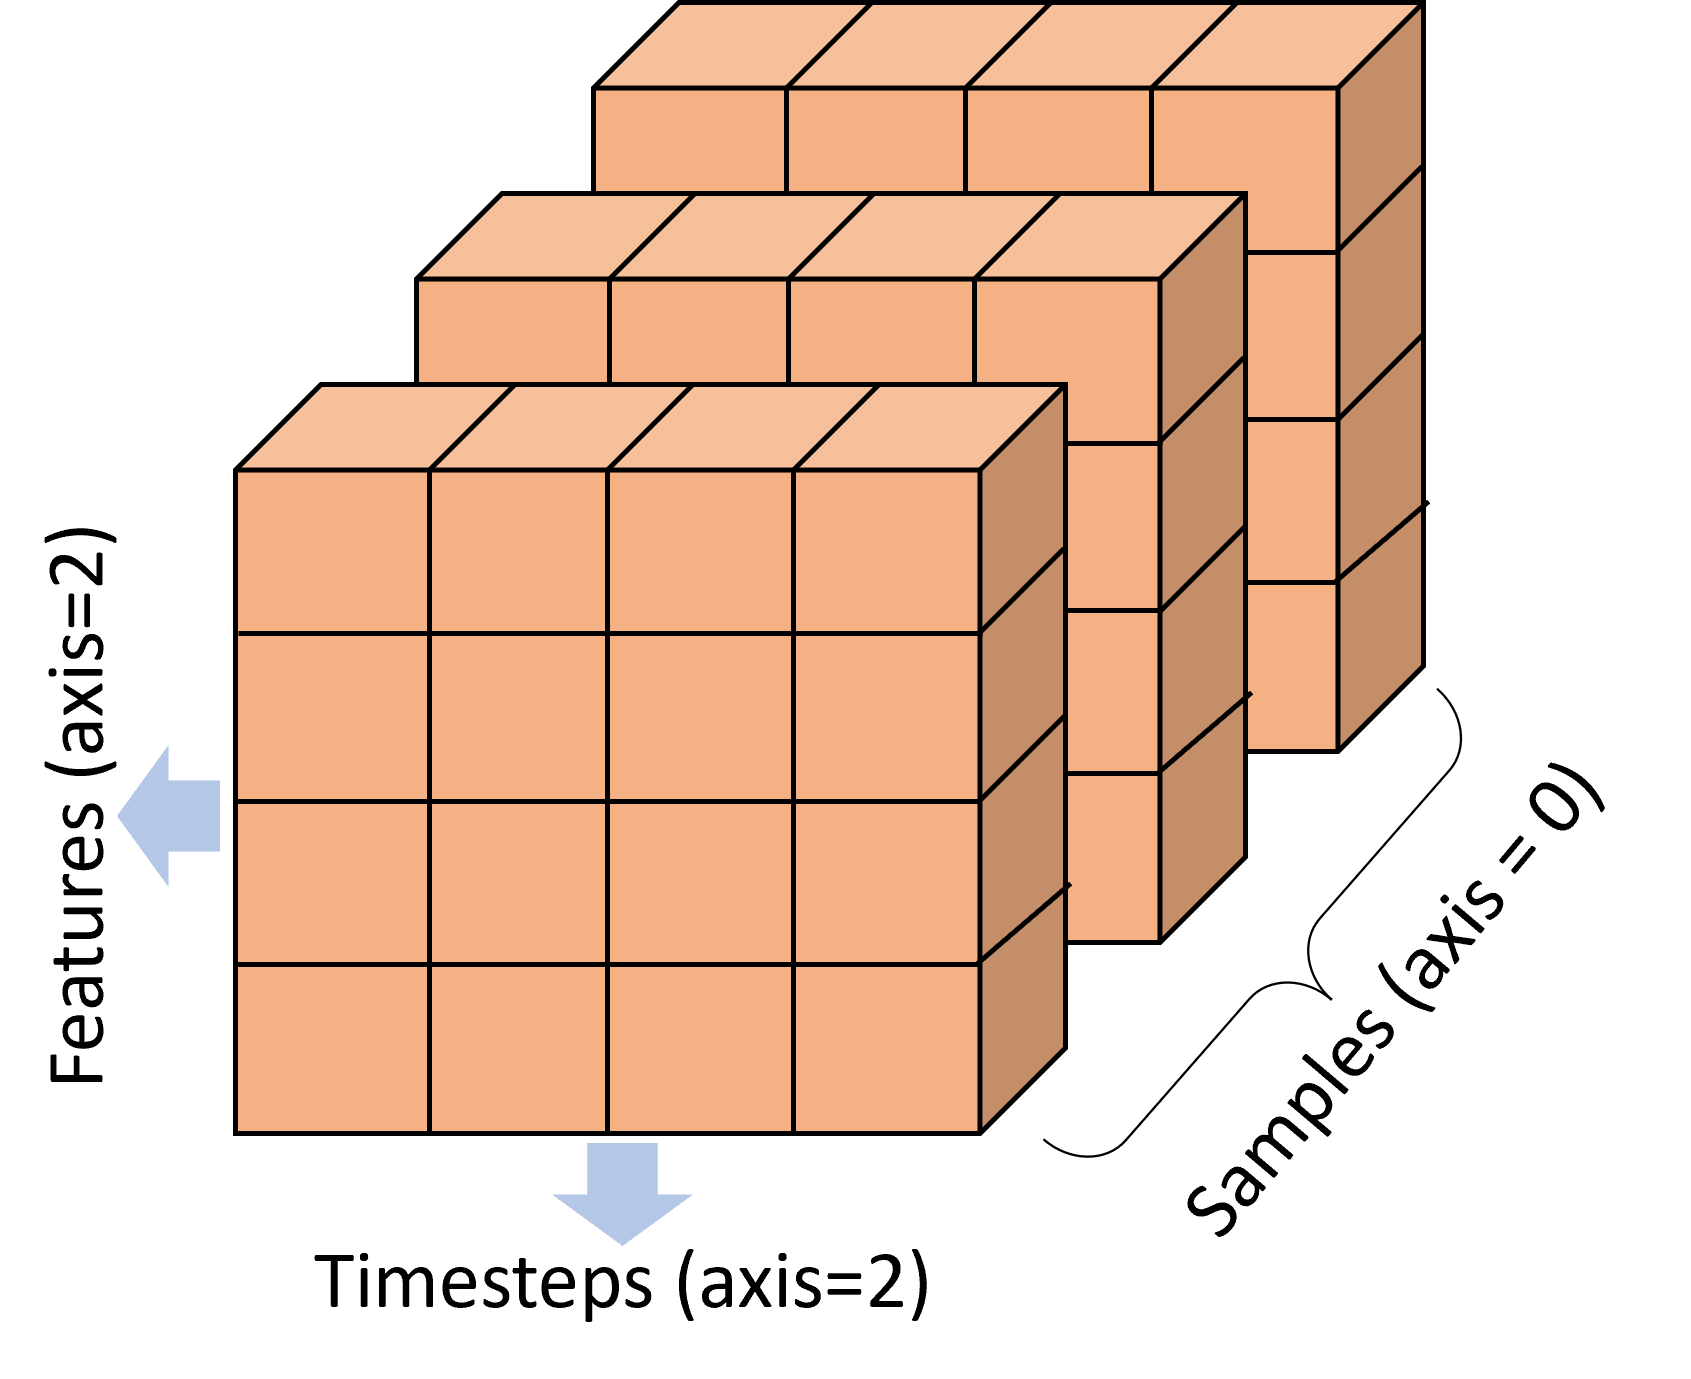
\includegraphics[width=0.5\linewidth]{images/samples-features-timesteps.png}
    \caption{Time series data represented as 3D tensors}
    \label{fig:ts_3d_data}
\end{figure}
\begin{lstlisting}[language=Python]
# Simulating streamflow data
streamflow = np.random.random((100, 1,3650))
# Extract data for the first 5 locations and the first 365 days (1 year)
subset = streamflow[:5, 0, :365]
print(subset.shape)  # Output: (5, 1, 365)
\end{lstlisting}
\end{itemize}

\begin{itemize}
    \item \subsubsection{Example 4: Satellite Image Data} 
    Satellite images are typically stored as 3D tensors (height, width, channels) or 4D tensors (batch size, height, width, channels) for a collection of images.
    In a land-cover classification example dataset of 200 satellite images, each with a resolution of 128x128 pixels and three RGB channels, would be stored as a 4D tensor of shape \texttt{(200, 128, 128, 3)}, in the format \texttt{(samples, width, height, channels)} as shown in Figure \ref{fig:4d-image-tensor}.
    \begin{lstlisting}[language=Python]
# Simulating a batch of satellite images
satellite_images = np.random.random((200, 128, 128, 3))
# Extract the first 50 images
batch_images = satellite_images[:50]
print(batch_images.shape)  # Output: (50, 128, 128, 3)
\end{lstlisting}
\end{itemize}

\begin{figure}
    \centering
    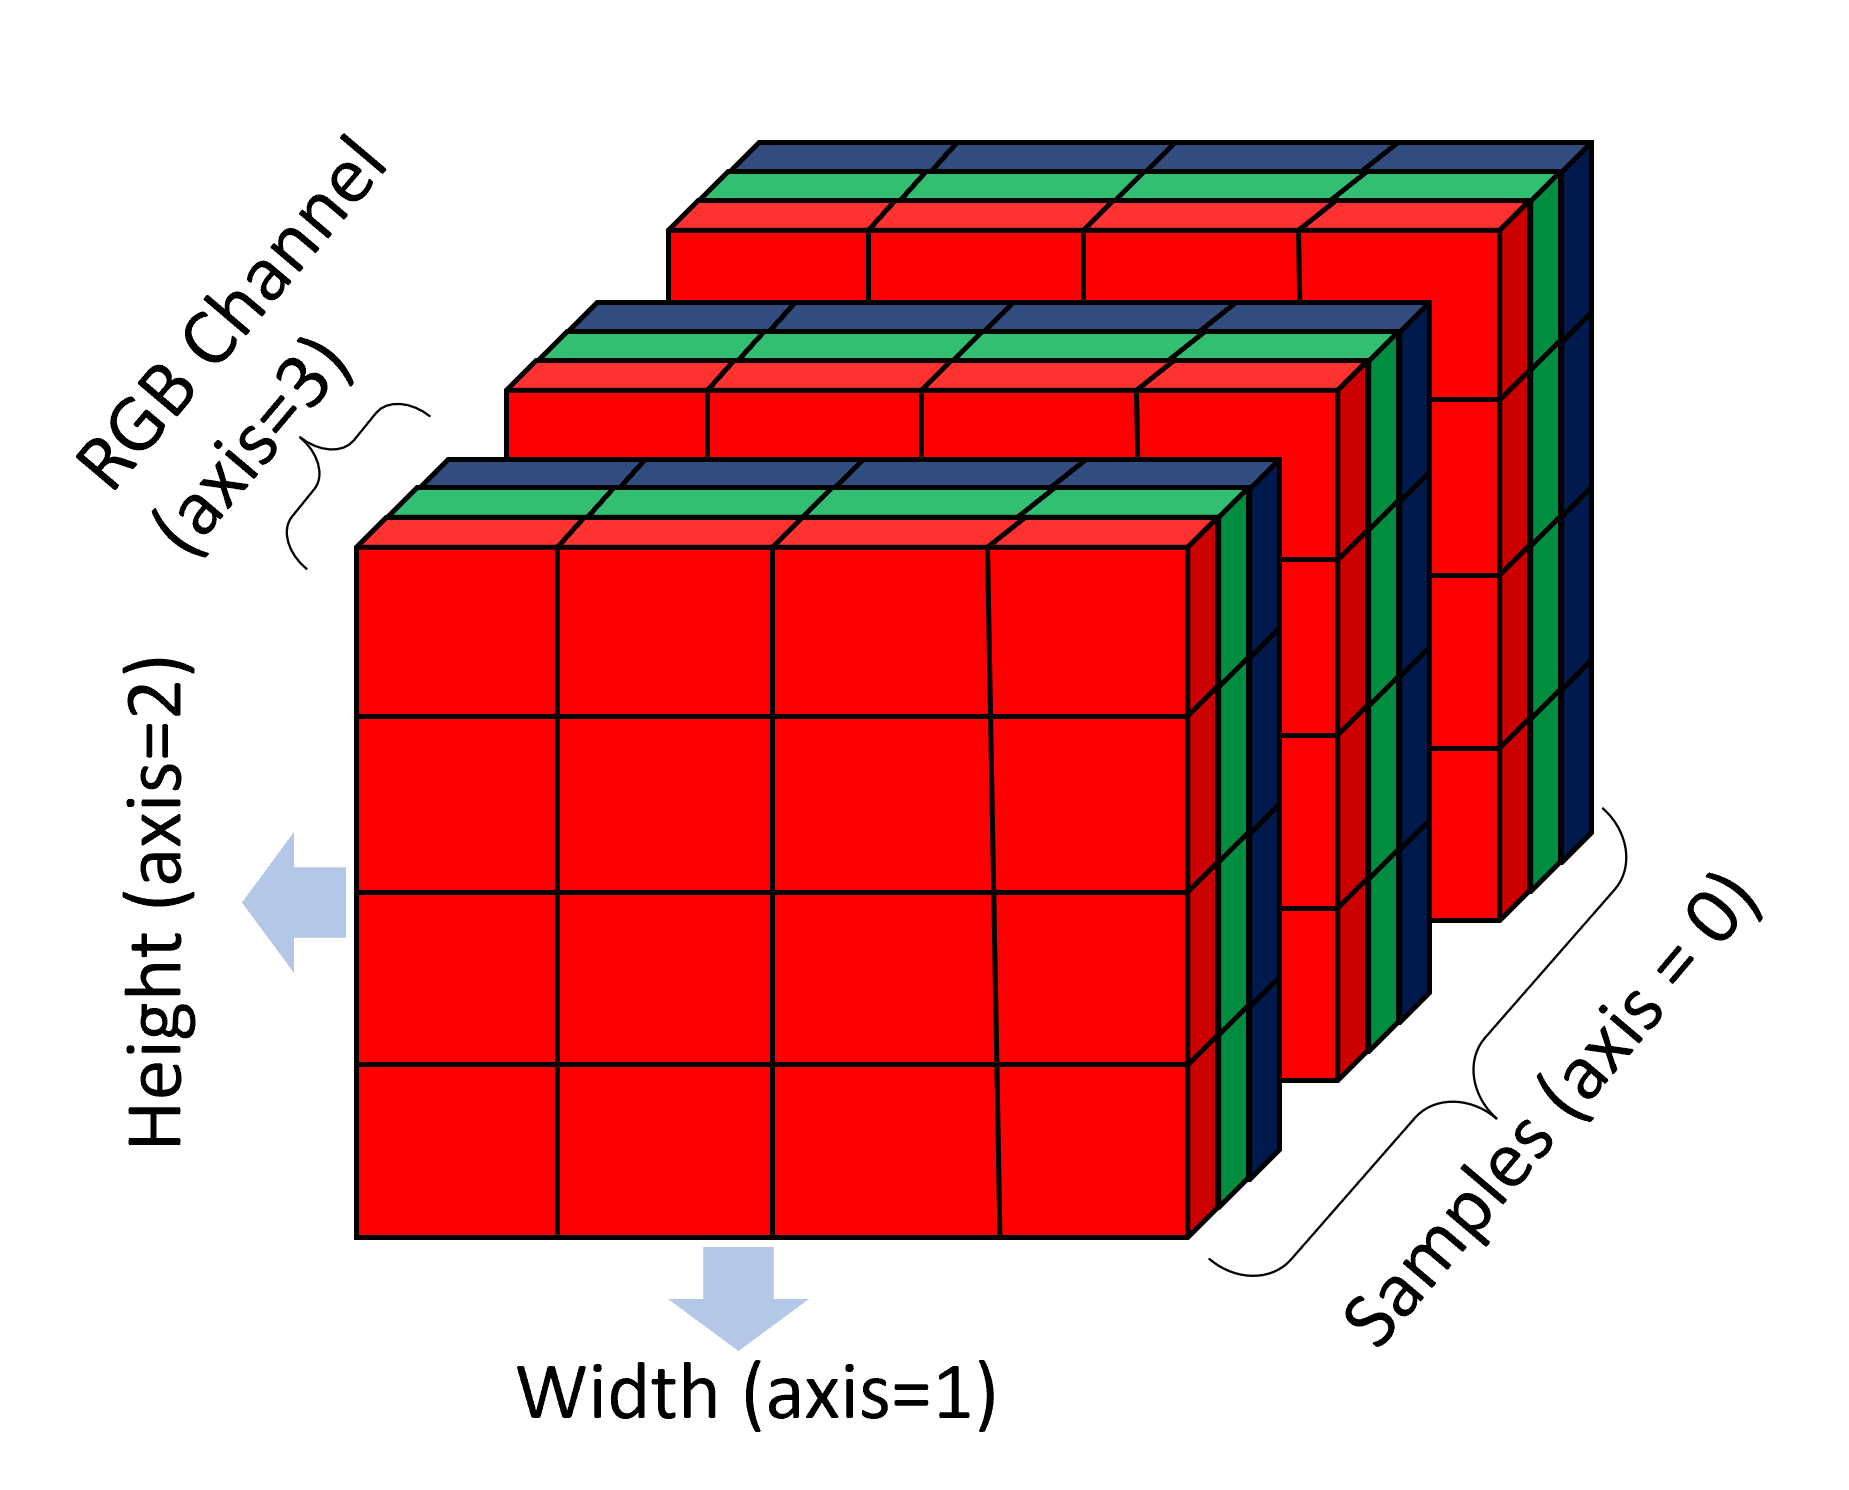
\includegraphics[width=0.5\linewidth]{images/4d-image-tensor.png}
    \caption{A 4D Image tensor data representation}
    \label{fig:4d-image-tensor}
\end{figure}





\section{Tensor Operations}


Much like computer programs are composed of simple operations on binary inputs (such as AND, OR, and XOR), deep learning models are built by applying tensor operations to numerical data. These operations are the foundation for all transformations a neural network performs. Tensor operations allow us to efficiently manipulate climate and earth science data, enabling tasks like precipitation prediction, satellite image classification, or hydrological time-series analysis.

In this section, we’ll cover the essential tensor operations—element-wise operations and broadcasting—through practical examples relevant to hydrology and remote sensing.

\subsection{Element-Wise Tensor Operations}

Element-wise operations are the simplest type of tensor operations. They involve applying a function independently to each element of a tensor or between corresponding elements of two tensors with the same shape.

\textbf{Example: Computing the Temperature Difference Between Two Grids}  
Suppose we have two temperature grids representing daily maximum and minimum temperatures (°C) over a region. These grids are stored as 2D tensors of shape \texttt{(100, 100)}, where rows and columns correspond to latitude and longitude. To compute the daily temperature range, we perform an element-wise subtraction.

\begin{lstlisting}[language=Python]
import numpy as np

# Simulated temperature grids
temp_max = np.random.random((100, 100)) * 40  # Max temperature
temp_min = np.random.random((100, 100)) * 20  # Min temperature

# Compute temperature range
temp_range = temp_max - temp_min
print(temp_range.shape)  # Output: (100, 100)
\end{lstlisting}

Each element in the \texttt{temp\_range} tensor corresponds to the temperature range at a specific grid cell.

Other common element-wise operations include addition, multiplication, and applying functions like \texttt{np.maximum()} or \texttt{np.exp()}.

---

\subsection{Broadcasting: Simplifying Operations on Tensors of Different Shapes}

In many real-world cases, tensors with different shapes need to interact. Broadcasting is a mechanism that allows smaller tensors to be automatically expanded to match the shape of larger tensors, without duplicating data in memory.

\textbf{Example: Adding a Rainfall Bias Across Multiple Regions}

Consider a dataset where daily rainfall data for 30 days is stored as a 2D tensor \texttt{rainfall} of shape \texttt{(30, 100)}, where rows represent days and columns represent regions. Suppose we want to add a constant bias correction to each region. The bias values are stored as a 1D tensor \texttt{bias} of shape \texttt{(100,)}.

\begin{lstlisting}[language=Python]
# Simulated rainfall data (mm) and bias correction
rainfall = np.random.random((30, 100)) * 50  # Daily rainfall
bias = np.random.random((100,)) * 2          # Bias for each region

# Add bias using broadcasting
corrected_rainfall = rainfall + bias
print(corrected_rainfall.shape)  # Output: (30, 100)
\end{lstlisting}

\textbf{How Broadcasting Works:}
1. The \texttt{bias} tensor of shape \texttt{(100,)} is reshaped to \texttt{(1, 100)} by adding a new axis.
2. The reshaped \texttt{bias} tensor is virtually repeated 30 times along the first axis to match the shape of \texttt{rainfall} (\texttt{(30, 100)}).
3. Element-wise addition is performed between the tensors.

\textit{Note:} Broadcasting happens at the algorithmic level and does not physically create new tensors, ensuring memory efficiency.

---

\subsubsection{A Practical Example in Remote Sensing}

Let’s consider satellite images with shape \texttt{(64, 3, 128, 128)}, representing a batch of 64 images with 3 color channels (RGB) and dimensions 128x128 pixels. We wish to normalize each pixel intensity by subtracting the mean intensity of its channel.

\begin{lstlisting}[language=Python]
# Simulated batch of images
images = np.random.random((64, 3, 128, 128)) * 255

# Mean intensity per channel
channel_mean = images.mean(axis=(0, 2, 3), keepdims=True)

# Normalize using broadcasting
normalized_images = images - channel_mean
print(normalized_images.shape)  # Output: (64, 3, 128, 128)
\end{lstlisting}

Here, the mean tensor \texttt{channel\_mean} is broadcasted to match the shape of \texttt{images}, enabling efficient subtraction across all pixels.

---

\subsection{Why Tensor Operations Matter in Hydrology}

Tensor operations are essential for:
\begin{itemize}
    \item \textbf{Analyzing Spatial Data:} Compute statistics, such as temperature ranges or precipitation anomalies, over grids.
    \item \textbf{Normalizing Datasets:} Prepare remote sensing images or time-series data for model training.
    \item \textbf{Efficient Computation:} Perform complex operations on large datasets without duplicating memory.
\end{itemize}

These operations are the building blocks for designing and training deep learning models tailored to hydrology and earth sciences.


\section{How Neural Networks Learn: Optimization Basics}

